\section{Quest�o 2}
\label{sec:q2}
%===============================================================================

Quest�o: Seja o sistema ARX (\ref{eq:q2arx}):

\begin{equation}
G_o(z)=\frac{2}{z-0.8}
\;\;
H_o(z)=\frac{z}{z-0.8}
\label{eq:q2arx}
\end{equation}

E com ruido branco com $ \lambda ^2 =0.1$.

\begin{itemize}
	\item Realize uma simulac�o aplicando na entrada um ruido branco com $\lambda ^2=1$.
	\item Plote 100 estimativas de $\hat{\theta}$, a elipse de 95\% de confianca e
	verifique o valor m�dio obtido e avalie a polarizac�o da estimativa.
	\item Repita o item anterior com $H(z)=1$.
\end{itemize}

\subsection{Item 1 e 2}
%===============================================================================

Para realizac�o desta simulac�o foi utilizado o script apresentado no Anexo 1.

Utilizando um ruido branco como entrada, com m�dia zero, e $\lambda ^2 = 1$, obtem-se 
os resultados apresentados na Figura (\ref{fig:q2_noise}).

\begin{figure}[htbp]
	\center
	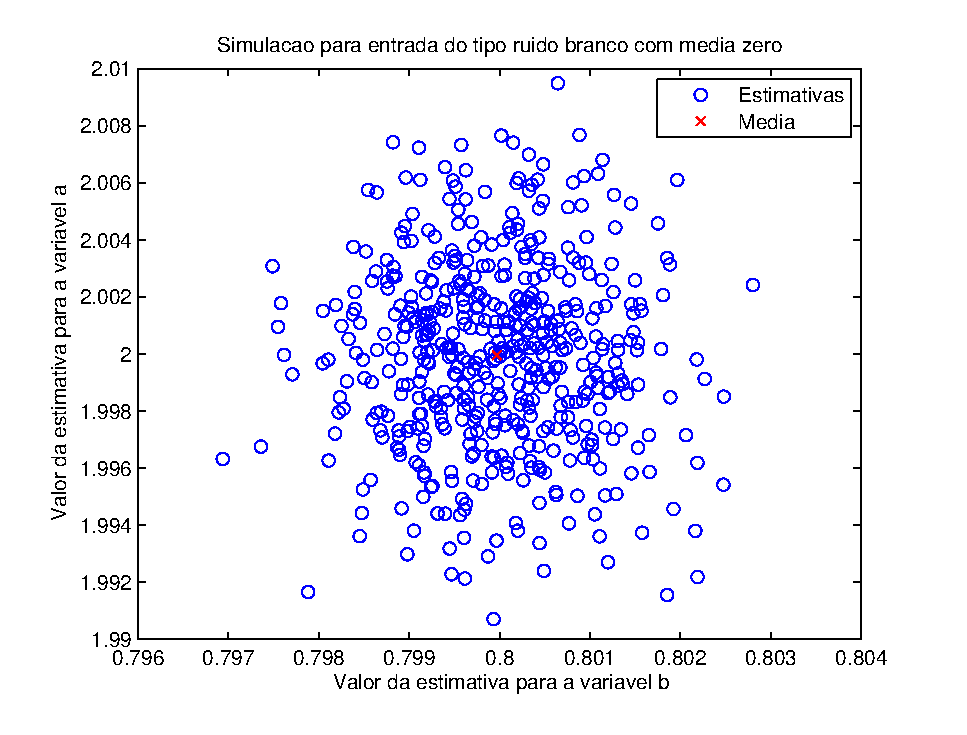
\includegraphics[width=0.98\columnwidth]{figures/q2_noise.eps}
	\caption{Entrada aleat�ria aplicada no processo para a identifica��o do sistema.}
	\label{fig:q2_noise}
\end{figure}

Observa-se que as estimativas em m�dia chegam relativamente pr�ximas ao valor real (a=2, b=0.8).
Desta forma conclui-se que n�o h� erro de polarizac�o. Quando o ruido inserido n�o possui m�dia
zero, h� a observac�o de erro de polarizac�o, como � apresentado na Figura (\ref{fig:q2_noise_pol}).

\begin{figure}[htbp]
	\center
	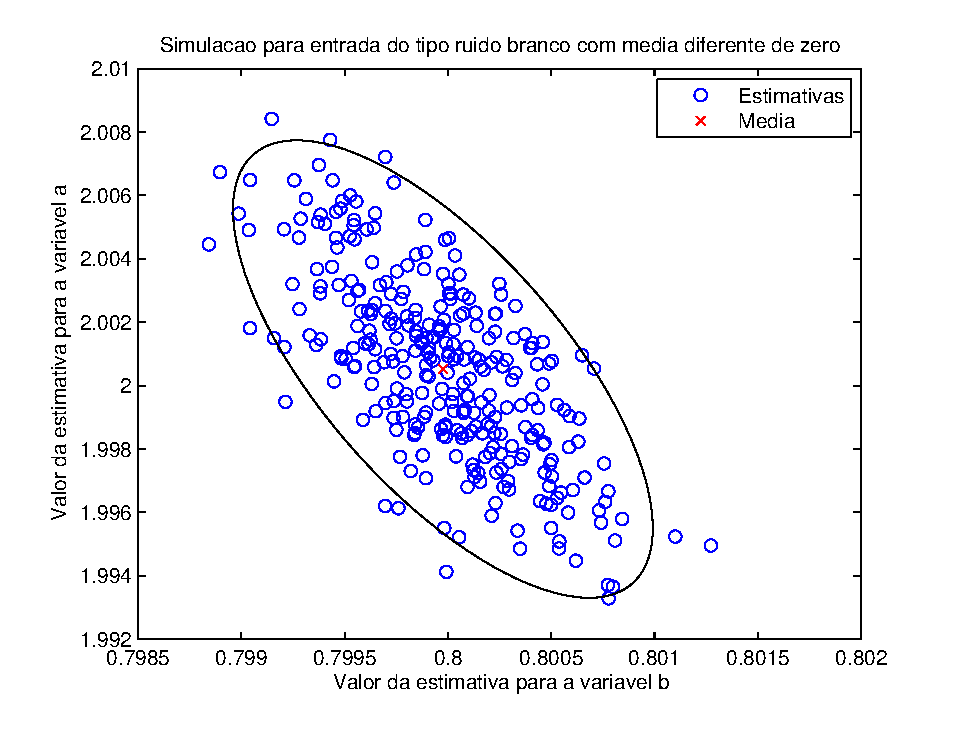
\includegraphics[width=0.98\columnwidth]{figures/q2_noise_pol.eps}
	\caption{Entrada aleat�ria aplicada no processo para a identifica��o do sistema. M�dia diferente de zero.}
	\label{fig:q2_noise}
\end{figure}

Neste caso, os valores m�dios encontrados foram b=0.8129 e a=2.003 e no caso onde a m�dia � zero, 
os valore estimados m�dios foram de a=1.9999 e b=0.8000.

\subsection{Item 3}
%===============================================================================

Na figura (\ref{fig:q2_noise_h1}) observa-se a simulac�o para o mesmo sistema do item anterior,
mas com o ruido branco sujeito a func�o de transferencia $H(z) = 1$.

\begin{figure}[htbp]
	\center
	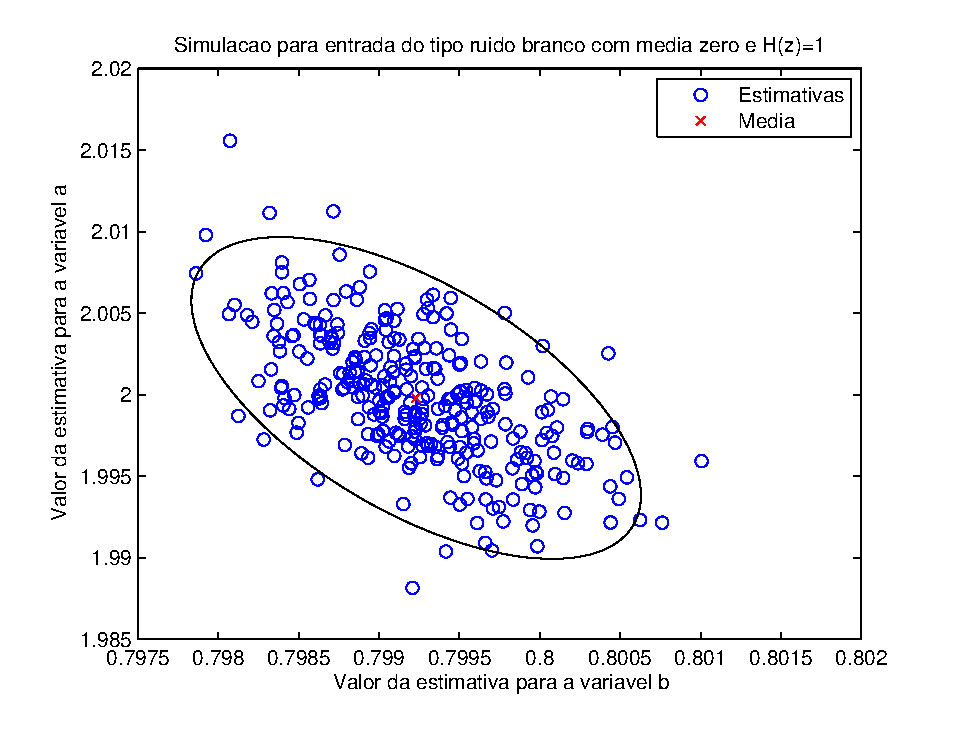
\includegraphics[width=0.98\columnwidth]{figures/q2_noise_h1.eps}
	\caption{Entrada aleat�ria aplicada no processo para a identifica��o do sistema. Ruido sujeito a
	$H(z)=1$.}
	\label{fig:q2_noise_h1}
\end{figure}

